\documentclass[12pt,a4paper]{article}

% ─── Packages ────────────────────────────────────────────────────────────────
\usepackage[T1]{fontenc}
\usepackage[utf8]{inputenc}
\usepackage{lmodern}
\usepackage[margin=2.5cm]{geometry}
\usepackage{graphicx}
\usepackage{float}
\usepackage{hyperref}
\usepackage{xcolor}
\usepackage{listings}
\usepackage{booktabs}
\usepackage{tabularx}
\usepackage{longtable}
\usepackage{amsmath}
\usepackage{amssymb}
\usepackage{enumitem}
\usepackage{fancyhdr}
\usepackage{titlesec}
\usepackage{microtype}
\usepackage{caption}
\usepackage{subcaption}
\usepackage{tikz}
\usetikzlibrary{shapes.geometric, arrows.meta, positioning, fit, backgrounds}

% ─── Hyperref setup ───────────────────────────────────────────────────────────
\hypersetup{
  colorlinks=true,
  linkcolor=blue!60!black,
  urlcolor=blue!60!black,
  citecolor=green!50!black,
  pdftitle={NPTEL Lecture Translation Pipeline},
  pdfauthor={Aditya Gaur},
}

% ─── Header / footer ──────────────────────────────────────────────────────────
\setlength{\headheight}{14pt}
\pagestyle{fancy}
\fancyhf{}
\fancyhead[L]{\small NPTEL Lecture Translation Pipeline}
\fancyhead[R]{\small BTP Report}
\fancyfoot[C]{\thepage}

% ─── Code listing style ───────────────────────────────────────────────────────
\lstset{
  basicstyle=\ttfamily\small,
  breaklines=true,
  frame=single,
  backgroundcolor=\color{gray!8},
  rulecolor=\color{gray!40},
  keywordstyle=\color{blue!70!black}\bfseries,
  commentstyle=\color{green!50!black}\itshape,
  stringstyle=\color{orange!80!black},
}

% ─── Section title formatting ─────────────────────────────────────────────────
\titleformat{\section}{\large\bfseries\color{blue!60!black}}{}{0em}{\thesection\quad}
\titleformat{\subsection}{\normalsize\bfseries\color{blue!40!black}}{}{0em}{\thesubsection\quad}
\titleformat{\subsubsection}{\normalsize\bfseries}{}{0em}{\thesubsubsection\quad}

% ─── TikZ pipeline arrow style ────────────────────────────────────────────────
\tikzset{
  block/.style={
    rectangle, rounded corners=4pt,
    draw=blue!50!black, fill=blue!8,
    text width=7em, minimum height=2.8em,
    text centered, font=\small\bfseries,
    line width=0.7pt,
  },
  optblock/.style={
    block, fill=orange!10, draw=orange!60!black, dashed,
  },
  arrow/.style={-{Stealth[length=6pt]}, thick, blue!50!black},
  note/.style={font=\scriptsize\itshape, text=gray!70!black},
}

% ═════════════════════════════════════════════════════════════════════════════
\begin{document}

% ─── Title page ───────────────────────────────────────────────────────────────
\begin{titlepage}
  \centering
  \vspace*{2cm}
  {\LARGE\bfseries NPTEL Lecture Translation Pipeline\\[0.4em]}
  {\large End-to-End Automatic Dubbing and Lip Synchronisation\\[0.4em]
   for Indian-Language Education\\[2em]}
  \rule{\linewidth}{0.5pt}\\[1em]
  {\large Bachelor of Technology Project Report\\[0.5em]}
  {\normalsize Department of Computer Science and Engineering\\[0.3em]
   IIIT Hyderabad\\[2em]}
  \rule{\linewidth}{0.5pt}\\[1em]
  {\large\bfseries Aryan Chugh\ \ (2023101016) \quad Aditya Gaur\ \ (2023101052)}\\[0.5em]
  {\normalsize Advisor: Prof.\ Vasudev Varma}\\[0.5em]
  {\normalsize\today}\\[3em]
  \begin{abstract}
    \noindent
    This report presents an end-to-end automatic video dubbing pipeline
    designed to translate English NPTEL lecture videos into Hindi,
    Telugu, and Odia — complete with dubbed audio, soft subtitles,
    voice cloning, and lip synchronisation.  The system chains
    seven distinct machine-learning and signal-processing stages:
    audio extraction, music separation (Demucs), speech-to-text
    (faster-Whisper), neural machine translation (GCP Cloud Translate / Gemini),
    text-to-speech (Google Cloud TTS Neural2), tone-colour voice cloning
    (OpenVoice v2), temporal alignment (RubberBand), and facial lip
    synchronisation (Wav2Lip).  Each component was evaluated against
    alternatives; the design decisions and performance trade-offs are
    documented here.  Sample outputs are available at:
    \href{https://drive.google.com/drive/folders/1_JSBJYKzM6jmwpKTSqcICVxC-7uiiQ1k?usp=drive_link}{Google Drive (sample outputs)}.
    The full source code is available at:
    \href{https://github.com/Aditya-Gaur26/multilingual_video_translation}{GitHub (codebase)}.
  \end{abstract}
\end{titlepage}

\tableofcontents
\newpage

% ═════════════════════════════════════════════════════════════════════════════
\section{Introduction}
% ═════════════════════════════════════════════════════════════════════════════

India's National Programme on Technology Enhanced Learning (NPTEL) provides
free video lectures from IITs and IIMs to millions of students.  However,
the content is delivered exclusively in English, creating a significant
access barrier for students whose first language is Hindi, Telugu, or Odia.

Manual dubbing of a one-hour lecture requires dozens of person-hours and
professional voice actors for every target language.  The goal of this
project is to automate this process entirely: given a raw English lecture
video, produce fully dubbed output videos for multiple Indian languages
without any human intervention.

The pipeline is implemented in Python and exposed through a browser-based
Streamlit interface.  All heavy computation (Whisper, OpenVoice, Wav2Lip) runs
on the local GPU.  Cloud API calls (GCP Translation, GCP TTS, Sarvam,
Gemini) are used for tasks where local models had lower quality.

\subsection{Design Goals}

\begin{enumerate}[leftmargin=*, label=\textbf{G\arabic*.}]
  \item \textbf{Fully automated} — no human intervention from raw video to
        dubbed output.
  \item \textbf{Temporally aligned} — dubbed speech must not overlap with
        subsequent English sentences; silence gaps must be preserved.
  \item \textbf{Voice-consistent} — dubbed audio should sound like the
        original lecturer, not a generic TTS robot.
  \item \textbf{Resource-constrained} — must run on a consumer GPU with
        4\,GB VRAM (NVIDIA GTX~1650\,Ti class).
  \item \textbf{Resumable} — intermediate results are cached; a crash at
        any stage does not require restarting from scratch.
\end{enumerate}

% ═════════════════════════════════════════════════════════════════════════════
\section{System Overview}
% ═════════════════════════════════════════════════════════════════════════════

\subsection{User Interface}

The pipeline is exposed through a Streamlit web application (\texttt{app.py}).
Figure~\ref{fig:ui} shows the main interface, which allows the user to upload
a lecture video, configure all pipeline stages through collapsible panels in
the sidebar, and monitor progress through real-time logs streamed to the browser.

\begin{figure}[H]
  \centering
  \IfFileExists{ui.png}{%
    \includegraphics[width=0.95\linewidth]{ui.png}%
  }{\IfFileExists{ui_screenshot.png}{%
    \includegraphics[width=0.95\linewidth]{ui_screenshot.png}%
  }{%
    \fbox{\parbox{0.9\linewidth}{\centering\vspace{9cm}
      [Place \texttt{ui.png} in the \texttt{report/} directory]\\[0.5em]
      Screenshot of the Streamlit web interface showing the video upload area,\\[0.3em]
      language selector, stage toggles, and real-time progress log.
      \vspace{9cm}}}%
  }}
  \caption{Streamlit UI --- users upload a video and configure each pipeline
           stage from the left sidebar before clicking Run.}
  \label{fig:ui}
\end{figure}

\subsection{High-Level Pipeline Architecture}

Figure~\ref{fig:pipeline} shows all stages and their data flow.

\begin{figure}[H]
\centering
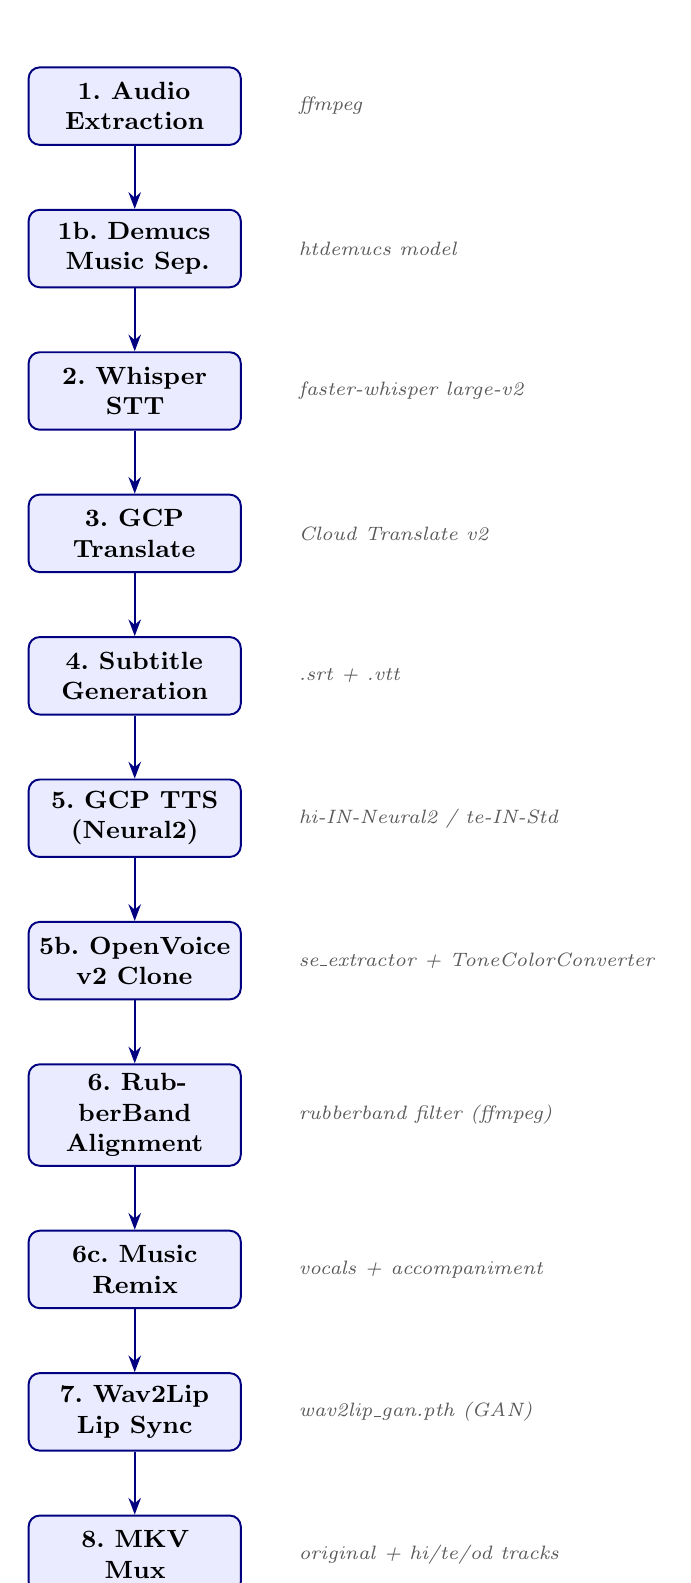
\begin{tikzpicture}[node distance=0.8cm and 1.8cm]

  % Column 1 — mandatory stages
  \node[block] (extract)  {1.\ Audio\\Extraction};
  \node[block, below=of extract] (demucs) {1b.\ Demucs\\Music Sep.};
  \node[block, below=of demucs]  (stt)    {2.\ Whisper\\STT};
  \node[block, below=of stt]     (trans)  {3.\ GCP\\Translate};
  \node[block, below=of trans]   (subs)   {4.\ Subtitle\\Generation};
  \node[block, below=of subs]    (tts)    {5.\ GCP TTS\\(Neural2)};
  \node[block, below=of tts]     (vc)     {5b.\ OpenVoice\\v2 Clone};
  \node[block, below=of vc]      (align)  {6.\ RubberBand\\Alignment};
  \node[block, below=of align]   (mix)    {6c.\ Music\\Remix};
  \node[block, below=of mix]     (wav2lip){7.\ Wav2Lip\\Lip Sync};
  \node[block, below=of wav2lip] (mux)    {8.\ MKV\\Mux};

  % Arrows down the main chain
  \foreach \from/\to in {
    extract/demucs, demucs/stt, stt/trans, trans/subs,
    subs/tts, tts/vc, vc/align, align/mix, mix/wav2lip, wav2lip/mux}
    \draw[arrow] (\from) -- (\to);

  % Side labels
  \node[note, right=0.6cm of extract]  {ffmpeg};
  \node[note, right=0.6cm of demucs]   {htdemucs model};
  \node[note, right=0.6cm of stt]      {faster-whisper large-v2};
  \node[note, right=0.6cm of trans]    {Cloud Translate v2};
  \node[note, right=0.6cm of subs]     {.srt + .vtt};
  \node[note, right=0.6cm of tts]      {hi-IN-Neural2 / te-IN-Std};
  \node[note, right=0.6cm of vc]       {se\_extractor + ToneColorConverter};
  \node[note, right=0.6cm of align]    {rubberband filter (ffmpeg)};
  \node[note, right=0.6cm of mix]      {vocals + accompaniment};
  \node[note, right=0.6cm of wav2lip]  {wav2lip\_gan.pth (GAN)};
  \node[note, right=0.6cm of mux]      {original + hi/te/od tracks};

\end{tikzpicture}
\caption{Pipeline stages and the technologies used at each step.  Optional
  stages (music separation, voice cloning, lip sync) are individually
  toggleable from the UI.}
\label{fig:pipeline}
\end{figure}

\subsection{Output Artefacts}

For each input video the pipeline produces:

\begin{table}[H]
\centering
\begin{tabularx}{\linewidth}{lX}
\toprule
\textbf{File} & \textbf{Description} \\
\midrule
\texttt{*\_dubbed.mkv}         & Multi-track MKV: original video, all audio and subtitle tracks \\
\texttt{*\_lipsync\_hi.mkv}    & Lip-synced video for Hindi \\
\texttt{*\_hi\_aligned.mp3}    & Dubbed Hindi audio aligned to original timing \\
\texttt{*\_hi\_mixed.mp3}      & Hindi audio with original background music re-added \\
\texttt{*\_hi.srt / .vtt}      & Hindi subtitle file \\
\texttt{lipsync\_debug/}       & Annotated frames showing face-detection bounding boxes \\
\texttt{.cache/}               & JSON snapshots for resuming interrupted runs \\
\bottomrule
\end{tabularx}
\caption{Output artefacts generated for a single input video (Hindi shown; analogous for Telugu and Odia).}
\end{table}

% ═════════════════════════════════════════════════════════════════════════════
\section{Stage~1: Audio Extraction}
% ═════════════════════════════════════════════════════════════════════════════

\textbf{Tool:} \texttt{ffmpeg}

The first stage strips the audio channel from the input video and writes a
16\,kHz mono WAV file.  This format is the industry standard for speech
recognition APIs and avoids downstream re-sampling artefacts.

\begin{lstlisting}[language=bash]
ffmpeg -i lecture.mp4 -ar 16000 -ac 1 lecture.wav
% 16 kHz mono WAV for downstream STT
\end{lstlisting}

All subsequent stages operate on this WAV file, never the original video,
until the final mux step.

% ═════════════════════════════════════════════════════════════════════════════
\section{Stage~1b: Music Separation (Demucs)}
% ═════════════════════════════════════════════════════════════════════════════

\textbf{Tool:} Meta Demucs (\texttt{htdemucs} model)

Many NPTEL lectures include opening and closing background music, title-card
transitions, or soft ambient audio.  If this is passed directly to the STT
engine, word error rate increases significantly.  Demucs separates the audio
into two stems:

\begin{itemize}
  \item \textbf{Vocals} (\texttt{vocals.wav}) — isolated lecturer speech fed
        to Whisper.
  \item \textbf{Accompaniment} (\texttt{no\_vocals.wav}) — background music
        held aside and re-mixed at the end.
\end{itemize}

\subsection{Why Demucs}

We evaluated three source-separation approaches:

\begin{table}[H]
\centering
\begin{tabularx}{\linewidth}{lXX}
\toprule
\textbf{Approach} & \textbf{Pros} & \textbf{Cons} \\
\midrule
Simple high-pass filter   & No dependencies    & Cannot separate vocals; damages speech \\
Spleeter (Deezer, 2019)   & Fast, simple API   & Lower separation quality, stale (Python~3.8 only) \\
\textbf{Demucs htdemucs}  & \textbf{State-of-art separation, single pip install, CPU fallback} & Slightly slower (~30\,s/min of audio) \\
\bottomrule
\end{tabularx}
\caption{Music separation alternatives evaluated.}
\end{table}

Demucs \texttt{htdemucs} was selected as the default. It is the only option
that reliably preserves voice quality while cleanly removing background music
in NPTEL videos.  The model (~80\,MB) is downloaded automatically on first
use.

\subsection{Auto-fallback}

If the STT stage returns ``no speech detected'' on the original audio (e.g.\
music-heavy intro), the pipeline automatically triggers Demucs even when the
user did not enable it, then retries transcription on the clean vocals stem.

% ═════════════════════════════════════════════════════════════════════════════
\section{Stage~2: Speech-to-Text (Whisper)}
% ═════════════════════════════════════════════════════════════════════════════

\textbf{Tool:} \texttt{faster-whisper} (CTranslate2 backend)\\
\textbf{Default model:} \texttt{large-v2}

\subsection{Engine Comparison}

Three STT backends were integrated and evaluated:

\begin{table}[H]
\centering
\begin{tabularx}{\linewidth}{lXXX}
\toprule
\textbf{Engine} & \textbf{Timestamp quality} & \textbf{Accuracy} & \textbf{Cost} \\
\midrule
Sarvam AI STT   & Sentence-level only        & Good for Indian-accented English & API (paid) \\
Google Gemini   & Sentence-level only        & Very high; hallucination risk on music & API (paid) \\
\textbf{Whisper large-v2} & \textbf{Word-level} & \textbf{Highest; native English} & \textbf{Free (local)} \\
\bottomrule
\end{tabularx}
\caption{STT engine comparison.  Whisper is the default.}
\end{table}

\textbf{Whisper} was chosen as the default for two critical reasons:
\begin{enumerate}
  \item \textbf{Word-level timestamps} — Whisper's cross-attention alignment
        produces per-word timestamps accurate to $\sim$100\,ms.  Gemini and
        Sarvam return only sentence-level start/end times, requiring
        heuristic interpolation for sub-sentence gaps.
  \item \textbf{Free and offline} — no API cost; runs entirely on the local GPU.
\end{enumerate}

\subsection{VAD Integration}

Whisper is run with the built-in Voice Activity Detection (VAD) filter
(\texttt{silero-vad} backend).  Parameters:

\begin{itemize}
  \item \texttt{min\_speech\_duration\_ms = 500}
  \item \texttt{speech\_pad\_ms = 200}
  \item \texttt{threshold = 0.5}
\end{itemize}

This suppresses hallucination on silent sections and reduces transcription
time by skipping non-speech regions.

\subsection{Duration-balanced chunking}

The word-level output is merged into sentence-level chunks using a
duration-balanced algorithm.  Each chunk is constrained to
$[5\text{s},\,13\text{s}]$ of original audio, with a target of 9\,s.
This ensures TTS segments are never so short that time-stretching would
be extreme, nor so long that a single segment spans multiple slides.

% ═════════════════════════════════════════════════════════════════════════════
\section{Stage~3: Translation}
% ═════════════════════════════════════════════════════════════════════════════

\textbf{Default:} Google Cloud Translation~v2 (REST API)\\
\textbf{Supported languages:} Hindi (\texttt{hi}), Telugu (\texttt{te}), Odia (\texttt{od})

\subsection{Engine Comparison}

\begin{table}[H]
\centering
\begin{tabularx}{\linewidth}{lXX}
\toprule
\textbf{Engine} & \textbf{Quality} & \textbf{Notes} \\
\midrule
Sarvam Translate  & High for Indian languages        & Limited context window; per-segment calls \\
Google Gemini     & High; context-aware              & Risk of ignoring glossary; slower batching \\
\textbf{GCP Cloud Translate} & \textbf{High; fast batch} & \textbf{Reliable, 100-segment batches, proven Indic quality} \\
\bottomrule
\end{tabularx}
\caption{Translation engine comparison.  GCP Cloud Translate is the default.}
\end{table}

GCP Cloud Translate was selected because it provides consistent quality at
high throughput (batches of 100 segments per API call) and has well-documented
Indic language support.  The pipeline uses \texttt{languageCode: hi}, \texttt{te},
or \texttt{or} (ISO 639-1 for Odia).

\subsection{Technical Term Preservation (Code-Mixing)}

NPTEL lectures contain a high density of English technical terms
(``neural network'', ``gradient descent'', ``CUDA'', etc.) that must
\emph{not} be translated — they should appear in English in the target-language
output, because equivalent terms are not standard in Hindi or Telugu pedagogy.

The pipeline implements a two-tier glossary:

\begin{enumerate}
  \item \textbf{Static glossary} — a curated list of $\sim$200 computer science,
        mathematics, and electronics terms hardcoded in \texttt{glossary.py}.
  \item \textbf{Dynamic glossary} — Gemini analyses the actual transcript and
        extracts domain-specific terms unique to that lecture (e.g.\
        ``backpropagation'', ``tokenisation'').
\end{enumerate}

Terms from the combined glossary are injected into the translation prompt as
explicit do-not-translate constraints.  A post-processing pass verifies
preservation and logs any missing terms.

% ═════════════════════════════════════════════════════════════════════════════
\section{Stage~4: Subtitle Generation}
% ═════════════════════════════════════════════════════════════════════════════

\textbf{Formats:} \texttt{.srt} and \texttt{.vtt} (Web Video Text Tracks)

Subtitle files are generated for all languages (English + all target
languages) directly from the segment timestamps produced by Whisper
(English) and propagated through translation (target languages).

Each subtitle line is word-wrapped at 42~characters per line and truncated
if the segment is shorter than the natural reading time.  Characters-per-second
thresholds were empirically tuned for Hindi Devanagari (which is visually
denser than Latin script).

The subtitle tracks are muxed as \emph{soft subtitles} into the final MKV
container, meaning they can be toggled on/off independently in any media
player (VLC, mpv, PotPlayer) without burning them into the video.

% ═════════════════════════════════════════════════════════════════════════════
\section{Stage~5: Text-to-Speech Synthesis}
% ═════════════════════════════════════════════════════════════════════════════

\textbf{Default:} Google Cloud TTS (\texttt{gcptts\_vc} engine = GCP Neural2 + OpenVoice~v2)

Each translated segment is synthesised into a short audio clip (~2--15\,s).
The output is one audio file per segment, e.g.\ \texttt{seg\_0001.mp3}.

\subsection{TTS Engine Comparison}

Five engines were integrated and tested:

\begin{table}[H]
\centering
\begin{tabularx}{\linewidth}{lXXX}
\toprule
\textbf{Engine} & \textbf{Voice quality} & \textbf{Indic language support} & \textbf{Requires} \\
\midrule
edge-tts (Microsoft)     & Neural, good  & Hindi, Telugu     & Free, online \\
Sarvam TTS               & Very good     & Hi/Te/Od          & Sarvam API key \\
Coqui XTTS~v2 (local)    & High; voice cloning built-in & Limited Indic & 6\,GB\,VRAM, slow \\
GCP TTS Standard         & Moderate      & Hi/Te             & GCP key \\
\textbf{GCP TTS Neural2} & \textbf{Highest naturalness} & \textbf{Hi/Te (Neural2/Standard)} & \textbf{GCP key} \\
\bottomrule
\end{tabularx}
\caption{TTS engine comparison.  GCP Neural2 is the default for Hindi; Standard for Telugu (Neural2 unavailable for \texttt{te-IN}).}
\end{table}

GCP TTS Neural2 was selected because it is the same WaveNet-based architecture
used by YouTube's auto-dubbing pipeline.  The specific voice models are:

\begin{itemize}
  \item Hindi: \texttt{hi-IN-Neural2-B} (male) / \texttt{hi-IN-Neural2-C} (female)
  \item Telugu: \texttt{te-IN-Standard-B} (male) / \texttt{te-IN-Standard-A} (female)
  \item Odia: GCP does not support \texttt{or-IN} → falls back to Sarvam TTS
\end{itemize}

\subsection{Duration-Aware SSML Rate Control}

Rather than synthesising at a fixed rate and always time-stretching afterwards,
the pipeline first estimates the natural duration of the TTS output using a
characters-per-second (CPS) model:

\begin{equation}
  r = \text{clamp}\!\left(\frac{N_\text{chars}}{t_\text{target} \times \text{CPS}},\; 0.65,\; 1.75\right)
\end{equation}

where $N_\text{chars}$ is the character count of the target-language text,
$t_\text{target}$ is the original segment duration in seconds, and
$\text{CPS} = 12.0$ for Hindi Devanagari.  The result is passed as
an SSML \texttt{<prosody rate="...">} attribute.  This two-pass approach
reduces the time-stretch ratio needed in Stage~6, improving final audio
naturalness.

% ═════════════════════════════════════════════════════════════════════════════
\section{Stage~5b: Voice Cloning (OpenVoice~v2)}
% ═════════════════════════════════════════════════════════════════════════════

\textbf{Tool:} MyShell OpenVoice~v2 (\href{https://github.com/myshell-ai/OpenVoice}{GitHub})\\
\textbf{Model size:} $\sim$300\,MB, auto-downloaded from HuggingFace

Even after Neural2 TTS, the dubbed audio sounds like a generic GCP voice.
OpenVoice~v2 is a \emph{language-agnostic} tone-colour transfer model that
re-tones the TTS output to sound like the original lecturer.

\subsection{How OpenVoice~v2 Works}

\begin{enumerate}
  \item A \textbf{speaker encoder} (similar to GE2E/d-vector) maps any
        audio clip to a 256-dimensional embedding that captures timbre,
        resonance, and voice quality — independent of linguistic content.
  \item The \textbf{ToneColorConverter} (a neural vocoder) re-synthesises
        the TTS audio using the source segment's \emph{content} but the
        reference lecturer's \emph{tone colour}.
\end{enumerate}

\subsection{Reference Clip Extraction}

A high-quality 30-second voiced reference clip is extracted automatically
from the lecture using Silero-VAD:

\begin{enumerate}
  \item The lecture is divided into three temporal zones: 15--30\%, 40--60\%,
        and 65--80\% through the video.
  \item Silero-VAD detects voiced speech frames in each zone.
  \item $\sim$10\,s of clean speech per zone is concatenated → 30\,s total.
  \item The result is resampled to 22\,050\,Hz mono (OpenVoice's required format)
        and bandpass-filtered (80--8000\,Hz) to remove low-frequency rumble and
        high-frequency hiss.
\end{enumerate}

Sampling across multiple zones rather than a single window ensures the
embedding captures the lecturer's voice across different speaking styles,
energy levels, and topic contexts.

\subsection{Per-Segment Conversion}

Voice cloning is applied \emph{per segment} (not on the full concatenated
track) because:
\begin{itemize}
  \item Each segment is short, focused, uninterrupted speech — ideal for
        the VAD inside the speaker encoder.
  \item The reference speaker embedding is computed once and cached in
        memory for the full run.
  \item The source embedding (per TTS segment) is computed fresh and
        immediately freed, keeping VRAM usage bounded.
\end{itemize}

Segments shorter than 0.5\,s are skipped (insufficient voiced frames for
reliable embedding extraction).

\subsection{Quality Verification}

After conversion, \textbf{Resemblyzer} computes the cosine similarity
between the converted output and the reference embedding.  This metric
is logged for every segment; segments with similarity below 0.65 are
flagged so the user can inspect them.

% ═════════════════════════════════════════════════════════════════════════════
\section{Stage~6: Temporal Alignment}
% ═════════════════════════════════════════════════════════════════════════════

\textbf{Tool:} RubberBand via \texttt{ffmpeg} \texttt{rubberband} audio filter

Translated speech is intrinsically longer than English in most Indian languages
(Hindi tends to be 15--25\% longer per sentence).  The aligner time-stretches
each TTS clip so it fits exactly within the original segment's time window.

\subsection{Rubber Band vs.\ ffmpeg \texttt{atempo}}

\begin{table}[H]
\centering
\begin{tabularx}{\linewidth}{lXX}
\toprule
\textbf{Method} & \textbf{Pros} & \textbf{Cons} \\
\midrule
\texttt{ffmpeg atempo}  & Simple; built-in & Phase-vocoder artefacts on speech; degrades formants \\
\textbf{RubberBand}     & \textbf{Phase-vocoder; pitch + formant preserving} & Requires \texttt{librubberband} package \\
\bottomrule
\end{tabularx}
\caption{Time-stretching method comparison.  RubberBand is the default.}
\end{table}

RubberBand's \texttt{formant=preserved} option maintains vowel quality even
at extreme stretch ratios, which is critical for Indic speech where vowel
length is phonemically distinctive.

\subsection{Bounds and Padding}

The tempo ratio is clamped to $[0.55,\,1.60]$.  When the TTS audio is
so long that even a 1.6$\times$ speedup cannot fit it in the window,
it is hard-truncated.  When it is shorter than the window even after
maximum slow-down, silence padding is inserted.

\subsection{Pitch Shift Post-processing}

After alignment, a separate pitch-shift step (via \texttt{ffmpeg rubberband})
adjusts the dubbed audio to match the original lecturer's measured average
pitch (extracted from the voice analysis stage).  This prevents the jarring
sensation of a lecturer who suddenly changes pitch between languages.

% ═════════════════════════════════════════════════════════════════════════════
\section{Stage~6c: Music Remix}
% ═════════════════════════════════════════════════════════════════════════════

The accompaniment stem saved by Demucs is mixed back with the aligned
dubbed audio using \texttt{ffmpeg amix}:

\begin{lstlisting}[language=bash]
ffmpeg -i dubbed_vocals.mp3 -i accompaniment.wav \\
  -filter_complex "[0:a][1:a]amix=inputs=2:duration=first:weights=1 0.18" \\
  output_mixed.mp3
\end{lstlisting}

The accompaniment weight (0.18) is calibrated so background music is
audible but does not overpower speech.  A loudness check is run first:
if the accompaniment energy is near $-\infty$\,dB (silence), the mix step
is skipped to avoid re-encoding the audio needlessly.

% ═════════════════════════════════════════════════════════════════════════════
\section{Stage~7: Lip Synchronisation (Wav2Lip)}
% ═════════════════════════════════════════════════════════════════════════════

\textbf{Tool:} Wav2Lip (Prajwal et al., 2020) with GAN checkpoint (\texttt{wav2lip\_gan.pth}, 436\,MB)

Wav2Lip is a Generative Adversarial Network that animates a speaker's mouth
in video to match a provided audio track.  It re-renders only the lower-face
region in each frame, blending seamlessly with the unchanged upper face and
background.

\subsection{Checkpoint Selection}

\begin{table}[H]
\centering
\begin{tabularx}{\linewidth}{lXX}
\toprule
\textbf{Checkpoint} & \textbf{Pros} & \textbf{Cons} \\
\midrule
\texttt{wav2lip.pth}       & Best sync accuracy              & Slight blurriness in lower face \\
\textbf{\texttt{wav2lip\_gan.pth}} & \textbf{Higher visual quality (GAN-sharpened)} & Marginally lower sync precision \\
\bottomrule
\end{tabularx}
\caption{Wav2Lip checkpoint comparison.  The GAN checkpoint is the default.}
\end{table}

\subsection{Segment-Aware Processing}

NPTEL lecture videos frequently switch between a camera shot of the lecturer
and a slide view (no face).  Running Wav2Lip on the full video fails
immediately when it encounters a slide frame.

The pipeline implements segment-aware processing:

\begin{enumerate}
  \item \textbf{Face detection scan:} the video is sampled at 0.5\,s intervals
        using the S3FD face detector.  Results are merged into segments of type
        \texttt{has\_face=True/False}.
  \item \textbf{Face segments} are passed to Wav2Lip.
  \item \textbf{Slide segments} use a simple ffmpeg audio-swap (no face
        animation needed).
  \item All processed clips are concatenated with ffmpeg.
\end{enumerate}

\subsection{RAM-Constrained Frame Processing}

Wav2Lip's \texttt{inference.py} loads the \emph{entire} video into a Python
list before processing.  For a 2-minute 1080p face segment this requires
$\approx 9.5$\,GB of RAM.  Two optimisations were implemented:

\begin{enumerate}
  \item \textbf{Pre-scale to 720p} — since Wav2Lip internally resizes every
        detected face crop to $96 \times 96$ before inference, there is no
        quality gain from feeding 1080p input.  ffmpeg scales the clip to
        $\leq 720$\,px height before calling \texttt{inference.py}.

  \item \textbf{$\leq$30\,s sub-chunks} --- clips longer than 30\,s are split into
        sub-chunks of exactly 30\,s, processed independently (each requiring
        $\approx 2$\,GB RAM), then concatenated.
\end{enumerate}

\subsection{Face Detection Robustness}

The original Wav2Lip code raises \texttt{ValueError: Face not detected} as
soon as any single frame has no detection.  The patched version:

\begin{enumerate}
  \item Collects all per-frame detection results first.
  \item Forward-fills missing detections from the nearest preceding valid detection.
  \item Backward-fills any remaining leading \texttt{None}s.
  \item Only raises an error if \emph{every} frame lacks a face.
\end{enumerate}

\subsection{VRAM Budget (4\,GB GPU)}

\begin{table}[H]
\centering
\begin{tabularx}{\linewidth}{lX}
\toprule
\textbf{Parameter} & \textbf{Value} \\
\midrule
\texttt{resize\_factor}       & 1 (full resolution input after 720p pre-scale) \\
\texttt{wav2lip\_batch\_size} & 8 frames per forward pass \\
\texttt{face\_det\_batch\_size} & 1 (one frame at a time to avoid RAM spike) \\
\texttt{PYTORCH\_CUDA\_ALLOC\_CONF} & \texttt{expandable\_segments:True} \\
\bottomrule
\end{tabularx}
\caption{Wav2Lip parameters tuned for 4\,GB VRAM.}
\end{table}

% ═════════════════════════════════════════════════════════════════════════════
\section{Stage~8: MKV Multiplexing}
% ═════════════════════════════════════════════════════════════════════════════

\textbf{Tool:} \texttt{ffmpeg}

The final step assembles all streams into a single \texttt{.mkv} Matroska
container:

\begin{itemize}
  \item Video stream: original (or lip-synced MP4 for per-language outputs).
  \item Audio track 0: English original.
  \item Audio tracks 1–$n$: Hindi, Telugu, Odia dubbed tracks.
  \item Subtitle tracks: one per language (.srt muxed as ASS).
\end{itemize}

Using a soft multi-track container means one MKV file can be played in VLC
with any language audio and any subtitle combination selected at runtime,
without re-encoding.

% ═════════════════════════════════════════════════════════════════════════════
\section{Caching and Resumability}
% ═════════════════════════════════════════════════════════════════════════════

Every major stage writes its result as a JSON file to
\texttt{output/<video>/.cache/} before proceeding.  On the next run,
if a cache file is found for a stage it is loaded and that stage is skipped.
This means:

\begin{itemize}
  \item A crash after Whisper (the slowest step) does not require
        re-transcribing.
  \item Changing the TTS engine only reruns Stage~5 onwards.
  \item Different target languages can be added without re-running STT or
        translation for languages already completed.
\end{itemize}

% ═════════════════════════════════════════════════════════════════════════════
\section{Voice Analysis and Filler Preservation}
% ═════════════════════════════════════════════════════════════════════════════

\subsection{Voice Analysis}

Before TTS synthesis, \texttt{voice\_analyzer.py} extracts from the original
audio:

\begin{itemize}
  \item Speaking rate (words per second)
  \item Average pitch / fundamental frequency (F0)
  \item Pitch range (min/max Hz)
  \item Average loudness (dBFS)
  \item Inferred gender (from F0: $<165$\,Hz → male; $>165$\,Hz → female)
\end{itemize}

The pitch measurement feeds the post-alignment pitch-shift step.  The
speaking rate informs SSML rate estimation in the TTS stage.

\subsection{Filler Preservation}

Lecturers naturally use hesitation markers (\texttt{um}, \texttt{uh},
\texttt{ah}, \texttt{hmm}, etc.) that contribute to natural speech rhythm.
The pipeline detects these in the Whisper word-level output and stores their
timing.  The TTS stage can optionally re-inject them as pauses in the dubbed
audio using SSML \texttt{<break>} tags, preserving the lecturer's natural
rhythm in the dubbed output.


\section{Sample Outputs}
% ═════════════════════════════════════════════════════════════════════════════

Sample output videos demonstrating the full pipeline on NPTEL lecture clips
are publicly available at:

\begin{center}
  \url{https://drive.google.com/drive/folders/1_JSBJYKzM6jmwpKTSqcICVxC-7uiiQ1k?usp=drive_link}
\end{center}

\noindent The complete source code for this project is hosted on GitHub:

\begin{center}
  \url{https://github.com/Aditya-Gaur26/multilingual_video_translation}
\end{center}



% ═════════════════════════════════════════════════════════════════════════════
\section{Limitations and Future Work}
% ═════════════════════════════════════════════════════════════════════════════

\begin{enumerate}[leftmargin=*, label=\textbf{L\arabic*.}]
  \item \textbf{Odia TTS quality} — GCP does not support \texttt{or-IN}
        Neural2 voices.  The Sarvam fallback is lower quality than Hindi/Telugu.
        Future work: fine-tune a local VITS model on Odia data.

  \item \textbf{Lip sync on partial faces} — Wav2Lip degrades on side-profile
        shots or when the lecturer turns away.  The bounding-box interpolation
        patch mitigates but does not eliminate this.

  \item \textbf{Slide-text translation} — text embedded in slide images
        (equations, code snippets) is not translated.  OCR + overlay rendering
        would be required.

  \item \textbf{Multi-speaker videos} — the current pipeline assumes a single
        speaker.  Panel discussions or Q\&A segments with multiple speakers
        would require speaker diarisation.

  \item \textbf{Gender-adaptive TTS} — voice gender is currently hardcoded
        to male.  Adding automatic gender detection from the voice profile
        would improve naturalness for female lecturers.
\end{enumerate}

\end{document}
